\scanpage{21}

\deleted{$(x_1-x_2)(x_3$}
\[
\prod_{\unsure{i\ne j}}(x_i-x_j)=\prod_i\left(\frac{f(x)}{\unsure{x_j|x}-x_i}\right)_{x\to x_i}=\prod_i f'(x_i).
\]
\margin{\figure{\begin{tikzpicture}[x=1cm,y=1cm]
\node[anchor=west] at (0.3,1.5) {$ (\unsure{y|x}+u)^3+a(y+u)^2 $};
\node at (1.7,0.8) {$3u+a$};
\node at (1.7,0.1) {$u=-\dfrac a3$};
\draw (-0.1,2.0) .. controls (0.5,1.5) and (0.4,0.2) .. (0.9,-0.3) .. controls (1.4,-0.5) and (2.5,-0.5) .. (3.2,-0.4);
\end{tikzpicture}}}
\[
f(x_i)=
\]
\[
3x^2+2ax+b
\]
\[
(3x_1^2+2ax_1+b)(3x_2^2+2ax_2+b)(3x_3^2+2ax_3+b)
\]
Supposons \uuline{$a=0$} \unsure{on trouve}
\margin{$x_1x_2\quad x_2x_3\quad x_3x_1$\par $x_1x_2\ x_2x_3$}
\[
j=-\frac{27c^2}{\Delta}
\]
\[
\begin{aligned}
\Delta=\prod(3x_i^2+b)&=27(x_1x_2x_3)^2+9b\bigl(\sum(x_1x_2)^2\bigr)\\
&\quad+3b^2\sum x_i^2\ \unsure{\}}+b^3
\end{aligned}
\]
\[
\deleted{=27c^{\unsure{3|2}}+9b(b^2-2\sum x_1^2x_2x_3}
\]
\[
(x_1x_2x_3)^2=c^2
\]
\[
\sum(x_1x_2)^2=(\sum x_1x_2)^2-2\sum x_1^2x_2x_3\ \unsure{=}
\]
\[
\sum x_i^2x_2x_3=(\sum x_1^2)(\sum x_2x_3
\]
\[
\boxed{\Delta=\deleted{\unsure{9|4}}b^3-27c^2}\quad ?
\]
\margin{$x_1^2x_2^2+$}
\[
\prod 3x_i^2+b
\]
\[
\deleted{(\sum\unsure{x^2})^2}
\]
\[
\cdot\ 3\sum(x_1x_2)^2+(\sum x_1x_2)(\sum x_i^2)
\]
\[
\deleted{\unsure{x_1x_2}}\qquad\deleted{x_1x_2}
\]
\mspage{20}
